\section*{Seminár 22}
\subsection*{Téma}
Geometria VI -- miš-maš
\subsection*{Ciele}
Precvičenie geometrických poznatkov, rôznorodné netradičné úlohy

\subsection*{Úlohy a riešenia}
\begin{tcolorbox}[breakable,notitle,boxrule=0pt,colback=light-gray,colframe=light-gray]\ul{22.1} [66-II-3] Dokážte, že obdĺžnik s~rozmermi $32 \times 120$ sa dá zakryť siedmimi zhodnými štvorcami so stranou 30.

\end{tcolorbox}

\rieh Štyrmi štvorcami so stranou 30 zrejme zakryjeme obdĺžnik $30\times 120$. Zvyšnú časť $2 \times 120$ rozdelíme na tri zhodné časti, konkrétne obdĺžniky $2 \times 40$, a ukážeme, ako každý z~nich (rovnako) pokryť jedným z~troch zvyšných štvorcov so stranou 30. Dosiahneme to, keď štvorec položíme na obdĺžnik tak, že obe uhlopriečky štvorca budú ležať na osiach súmernosti dotyčného obdĺžnika. Stačí potom ukázať, že obdĺžnik so stranou 2 vpísaný do štvorca podľa obr. 1 má druhú stranu dlhšiu ako 40. Jej dĺžka je zrejme $30\sqrt{2}-2$ (od uhlopriečky štvorca odčítame na každej strane 1 ako veľkosť výšky
\begin{center}
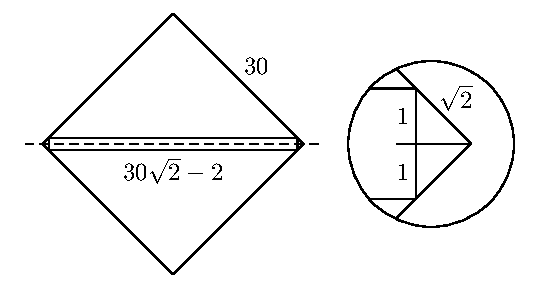
\includegraphics{obrazky/66K3} \\

Obr. 1
\end{center}
pravouhlého trojuholníka so stranami $2, \sqrt{2}, \sqrt{2}$, pozri zväčšenú časť obr. 1), takže stačí ukázať, že $30\sqrt{2}-2\geq 40$. To je ekvivalentné s~nerovnosťou $5\sqrt{2}\geq 7$, čiže $50 \geq 49$, čo je splnené. Daný obdĺžnik $32 \times 120$ teda naozaj možno zakryť siedmimi štvorcami so stranou 30.\\
\\
\begin{tcolorbox}[breakable,notitle,boxrule=0pt,colback=light-gray,colframe=light-gray]\ul{22.2} [60-S-2]  Daný je štvorec so stranou dĺžky 6\,cm. Nájdite množinu stredov všetkých priečok štvorca, ktoré ho delia na dva štvoruholníky, z~ktorých jeden má obsah 12\,cm$^2$. (Priečka štvorca je úsečka, ktorej krajné body ležia na stranách štvorca.)

\end{tcolorbox}

\rieh Ak priečka delí štvorec na dva štvoruholníky, musia ich koncové body ležať na protiľahlých stranách štvorca. V~takom prípade sú oba štvoruholníky lichobežníkmi alebo pravouholníkmi (pre potreby tohto riešenia budeme pravouholník považovať za špeciálny lichobežník). Označme daný štvorec $ABCD$, koncové body priečky označme $K$ a $L$. Predpokladajme, že bod $K$ leží na strane $AD$, potom bod $L$ leží na strane $BC$. Jeden zo štvoruholníkov $KABL$ a $KDCL$ má podľa zadania obsah 12\,cm$^2$; nech je to napr. lichobežník $KABL$.

Obsah lichobežníka vypočítame ako súčin jeho výšky s~dĺžkou strednej priečky. Výška je v~našom prípade rovná dĺžke strany štvorca, čiže 6\,cm. Jeho stredná priečka má teda dĺžku 2\,cm. Z~toho vyplýva, že stred úsečky $KL$ musí ležať na osi strany $AB$ vo
\begin{center}
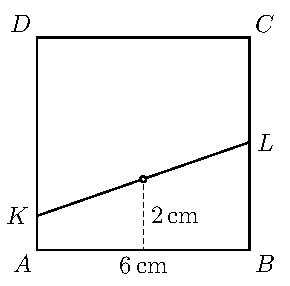
\includegraphics{obrazky/60S21} \ \ \ \ \ 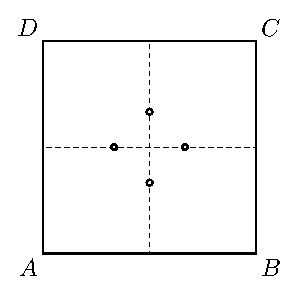
\includegraphics{obrazky/60S22} \\

Obr. 2 \hspace{130pt} Obr. 3
\end{center}
vzdialenosti 2\,cm od stredu strany $AB$ (obr. 2). Platí to aj naopak: Ak stred úsečky $KL$ leží v~opísanej polohe, bude štvoruholník $KABL$ lichobežník s~obsahom 12\,cm$^2$.

Ak budeme namiesto lichobežníka $KABL$ uvažovať lichobežník $KDCL$, vyjde stred priečky $KL$ na osi úsečky $CD$ vo vzdialenosti 2\,cm od stredu strany $CD$.

Ak priečka $KL$ spája body na stranách $AB$ a $CD$, dostaneme ďalšie dva možné body ležiace na spojnici stredov úsečiek $AD$ a $BC$. Hľadanú množinu teda tvoria štyri body, ktoré ležia na priečkach spájajúcich stredy protiľahlých strán štvorca vo vzdialenosti 1\,cm od jeho stredu (obr. 3).

\begin{tcolorbox}[breakable,notitle,boxrule=0pt,colback=light-gray,colframe=light-gray]\ul{22.4} [65-S-3] V~kružnici so stredom $S$ zostrojíme priemer $AB$ a ľubovoľnú naň kolmú tetivu $CD$. Zdôvodnite, prečo je obvod trojuholníka $ACD$ menší ako dvojnásobok obvodu trojuholníka $SBC$.

\end{tcolorbox}

\rieh Želaný vzťah medzi obvodmi trojuholníkov $ACD$ a $SBC$ vyplynie, keď pre dĺžky ich strán objavíme nerovnosti
$$|AC| < 2|SB|,\ \ \ \  |AD| < 2|SC|\ \ \ \  \text{a} \ \ \ \  |CD| < 2|BC|.$$
Prvé dve z~nich sú dôsledkom toho, že tetivy $AC$ a $AD$ danej kružnice sú kratšie ako jej priemer $AB$ (obr. 1), tretia nerovnosť zapísaná v~tvare $\frac{1}{2}|CD| < |BC|$ je nerovnosťou medzi dĺžkami odvesny a prepony dvoch zhodných pravouhlých trojuholníkov, na ktoré je trojuholník $BCD$ rozdelený priamkou $AB$, ktorá je totiž (vďaka predpokladu $AB \perp CD$) osou tetivy $CD$. Dodajme, že rovnako dobre možno využiť aj trojuholníkovú nerovnosť $|CD| < |BC| + |BD| = 2|BC|$.
\begin{center}
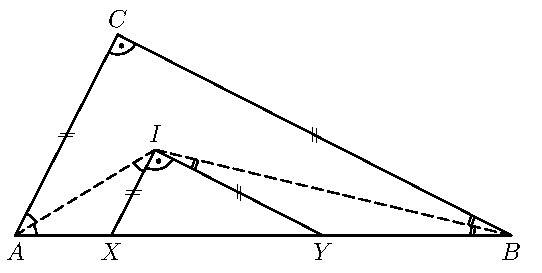
\includegraphics{obrazky/63S3}\\

Obr. 5
\end{center}
\textbf{Iné riešenie.} Označme $\alpha$ veľkosti vnútorných uhlov pri základni $AC$ rovnoramenného trojuholníka $SAC$. Potom jeho vonkajší uhol pri vrchole $S$, čiže uhol $CSB$, má veľkosť $2\alpha$, ktorú má aj uhol $CAD$, pretože polpriamka $AB$ je jeho osou (obr. 5). 2Rovnoramenné trojuholníky $ACD$ a $SCB$ sa tak zhodujú vo vnútorných uhloch pri svojich hlavných vrcholoch $A$ a $S$, a sú teda podobné. Preto je pomer ich obvodov rovný pomeru dĺžok ich ramien, a ten má naozaj hodnotu menšiu ako 2, lebo ramená trojuholníka $ACD$ sú kratšie ako priemer danej kružnice, zatiaľ čo ramená trojuholníka $SCB$ majú dĺžku jej polomeru.\\
\\
\begin{tcolorbox}[breakable,notitle,boxrule=0pt,colback=light-gray,colframe=light-gray]\ul{22.5} [59-S-2] Kružnice $k(S; 6\,\text{cm})$ a $l(O; 4\,\text{cm})$ majú vnútorný dotyk v~bode $B$. Určte dĺžky strán trojuholníka $ABC$, pričom bod $A$ je priesečník priamky $OB$ s~kružnicou $k$ a bod $C$ je priesečník kružnice $k$ s~dotyčnicou z~bodu $A$ ku kružnici $l$.

\end{tcolorbox}

\rieh Bod dotyku kružnice $l$ s~dotyčnicou z~bodu $A$ označme $D$ (obr. 6). Z~vlastností dotyčnice ku kružnici vyplýva, že uhol $ADO$ je pravý. Zároveň je pravý aj uhol
\begin{center}
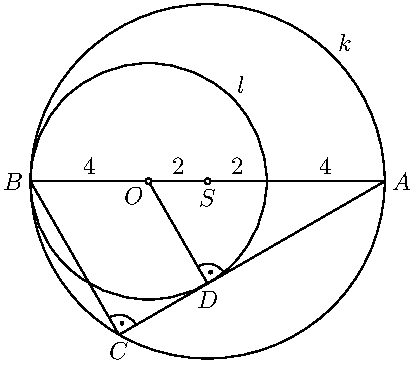
\includegraphics{obrazky/59S2}\\

Obr. 6
\end{center}
$ACB$ (Tálesova veta). Trojuholníky $ABC$ a $AOD$ sú tak podobné podľa vety $uu$, lebo sa zhodujú v~uhloch $ACB$, $ADO$ a v~spoločnom uhle pri vrchole $A$. Z~uvedenej podobnosti vyplýva
$$\frac{|BC|}{|OD|}=\frac{|AB|}{|AO|}. \ \ \ \  (1)$$
Zo zadaných číselných hodnôt vychádza $|OD| = |OB| = 4$\,cm, $|OS| = |SB| - |OB| = 2$\,cm, $|OA| = |OS| + |SA| = 8$\,cm a $|AB| = 12$\,cm. Podľa (1) je teda $|BC| : 4\,\text{cm} = 12 : 8$ a odtiaľ $|BC| = 6$\,cm. Z~Pytagorovej vety pre trojuholník $ABC$ nakoniec zistíme, že $|AC| = \sqrt{12^2 - 6^2}\,\text{cm}= 6$\,cm.\\
\\
\begin{tcolorbox}[breakable,notitle,boxrule=0pt,colback=light-gray,colframe=light-gray] \ul{22.6} [63-II-4]  Daný je konvexný štvoruholník $ABCD$ s bodom$E$ vnútri strany $AB$ tak, že platí $|\ma ADE| = |\ma DEC| = |\ma ECB|$. Obsahy trojuholníkov $AED$ a $CEB$ sú postupne 18\,cm$^2$ a 8\,cm$^2$ . Určte obsah trojuholníka $ECD$.
\end{tcolorbox}

\rieh Hľadaný obsah trojuholníka $ECD$ označme $S$. Uhol $DEC$ je striedavý s uhlami $ADE$ a $ECB$, odtiaľ $AD  \parallel EC$ a $ED \parallel BC$ (obr. 7). Trojuholníky $EDA$
\begin{center}
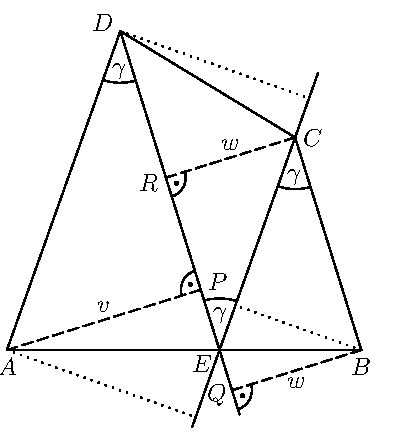
\includegraphics{obrazky/63K41}\\

Obr. 7
\end{center}
a $EDC$ majú spoločnú stranu $ED$, pomer ich obsahov je teda rovný pomeru prislúchajúcich výšok. Ak navyše postupne označíme $P, Q a R$ kolmé priemety vrcholov $A, B a C$ na priamku $DE$ a označíme $v = |AP|$, $w = |BQ| = |CR|$, dostaneme z podobných
pravouhlých trojuholníkov $AEP$ a $BEQ$ úmeru
$$\frac{18}{S}=\frac{v}{w}=\frac{|AE|}{|EB|}.$$
Analogicky pre trojuholníky $ECD$ a $ECB$ zistíme, že
$$\frac{8}{S}=\frac{|EB|}{|AE|}.$$
(V obr. 7 sú prislúchajúce priemety iba naznačené, ale jedná sa o ten istý výpočet
ako v predošlom odseku, len v ňom zameníme zodpovedajúce body $A\leftrightarrow B, C \leftrightarrow D$ a prislúchajúce obsahy trojuholníkov $AED$ a $BEC$.) Dokopy teda je $S : 8 = 18 : S$ čiže $S^2 = 144$, takže trojuholník $ECD$ má obsah $S = 12$\,cm$^2$ .





